\documentclass [xcolor=svgnames, t] {beamer} 
\usepackage[utf8]{inputenc}
\usepackage{booktabs, comment} 
\usepackage[absolute, overlay]{textpos} 
\usepackage{pgfpages}
\usepackage[font=footnotesize]{caption}
\useoutertheme{infolines} 

\AtBeginSection[]{
  \begin{frame}
  \vfill
  \centering
  \begin{beamercolorbox}[sep=8pt,center,shadow=true,rounded=true]{title}
    \usebeamerfont{title}\insertsectionhead\par%
  \end{beamercolorbox}
  \vfill
  \end{frame}
}


%\definecolor{brownbrown}{RGB}{56, 28, 0}
%\definecolor{brownred}{RGB}{228, 0, 43}

%\setbeamercolor{title in head/foot}{bg=brownred, fg=brownbrown}
%\setbeamercolor{author in head/foot}{bg=myuniversity}
\setbeamertemplate{page number in head/foot}{}
\usepackage{csquotes}


\usepackage{amsmath}
\usepackage[makeroom]{cancel}
\usepackage[absolute,overlay]{textpos}

%\usepackage{textpos}

\usepackage{tikz}

\usepackage{media9} 

\usetheme{Madrid}
%\definecolor{myuniversity}{RGB}{56, 28, 0}
%\usecolortheme[named=myuniversity]{structure}



\title[Viscosidad]{Clase No.12: Est\'atica de los fluidos}
\subtitle{Fuerzas sobre superficies planas, principios de flotaci\'on y equilibrio relativo de fluidos en movimiento}
\institute[]{Departamento de Ingenier\'ia Civil y Agr\'icola\\ Facultad de Ingenier\'ia  \\Universidad Nacional de Colombia - Sede Bogot\'a}
\titlegraphic{
\includegraphics[height=2.0cm]{escudoUnal.png}}
\author[LAM]{Luis Alejandro Morales \\ \href{https://lamhydro.github.io}{https://lamhydro.github.io}}


%\institute[]{Department of Earth, Environmental, and Planetary Sciences  \\Brown University}
\date{\today}


\addtobeamertemplate{navigation symbols}{}{%
    \usebeamerfont{footline}%
    \usebeamercolor[fg]{footline}%
    \hspace{1em}%
    \insertframenumber/\inserttotalframenumber
}

\begin{document}
\begin{frame}
\maketitle
\end{frame}


%%%%%%%%%%%%%%%%%%%%%%%%%%%%
\logo{\vspace{-0.2cm}
\includegraphics[height=0.8cm]{escudoUnal.png}~%
}
%%%%%%%%%%%%%%%%%%%%%%%%%%



\begin{frame}
\frametitle{Table of Contents}
\tableofcontents
\end{frame}

\section{Fuerzas sobre superficies curvas}
\begin{frame}{Fuerzas sobre superficies curvas: Aplicaciones}
Necesaria en la estimaci\'on de fuerzas sobre estructuras hidr\'aulicas curvas como:
\begin{itemize}
\item compuertas tipo tambor
\item compuertas radiales
\item Cara superior tipo par\'abola en presas
\end{itemize}
\begin{textblock*}{10.5cm}(1.0cm,4.3cm) % {block width} (coords)
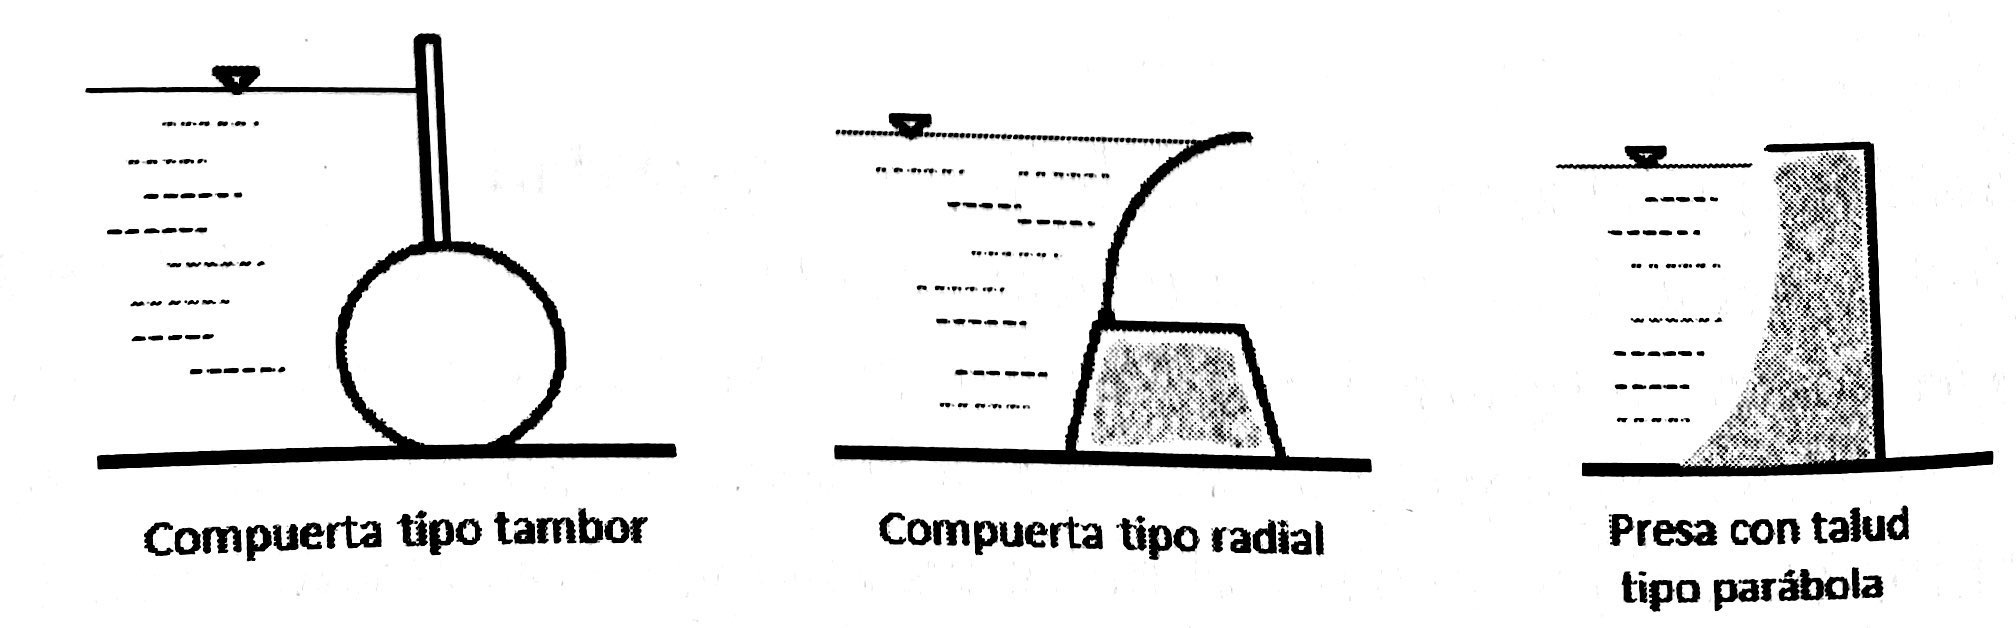
\includegraphics[width=\textwidth]{curb1}
\end{textblock*}
\end{frame} 

\begin{frame}{Fuerzas sobre superficies curvas: Fuerzas}
En una superficie curva sumergida, la fuerza hidroesti\'atica cambia de direcci\'on dependiendo de la posici\'on sobre la superficie. Para facilitar el c\'alculo, es necesario estimar las componentes horizontal $F_H$ y vertical $F_V$ de  la fuerza resultante $F_R$ sobre la superficie curva. 
\begin{textblock*}{6.5cm}(3.0cm,4.3cm) % {block width} (coords)
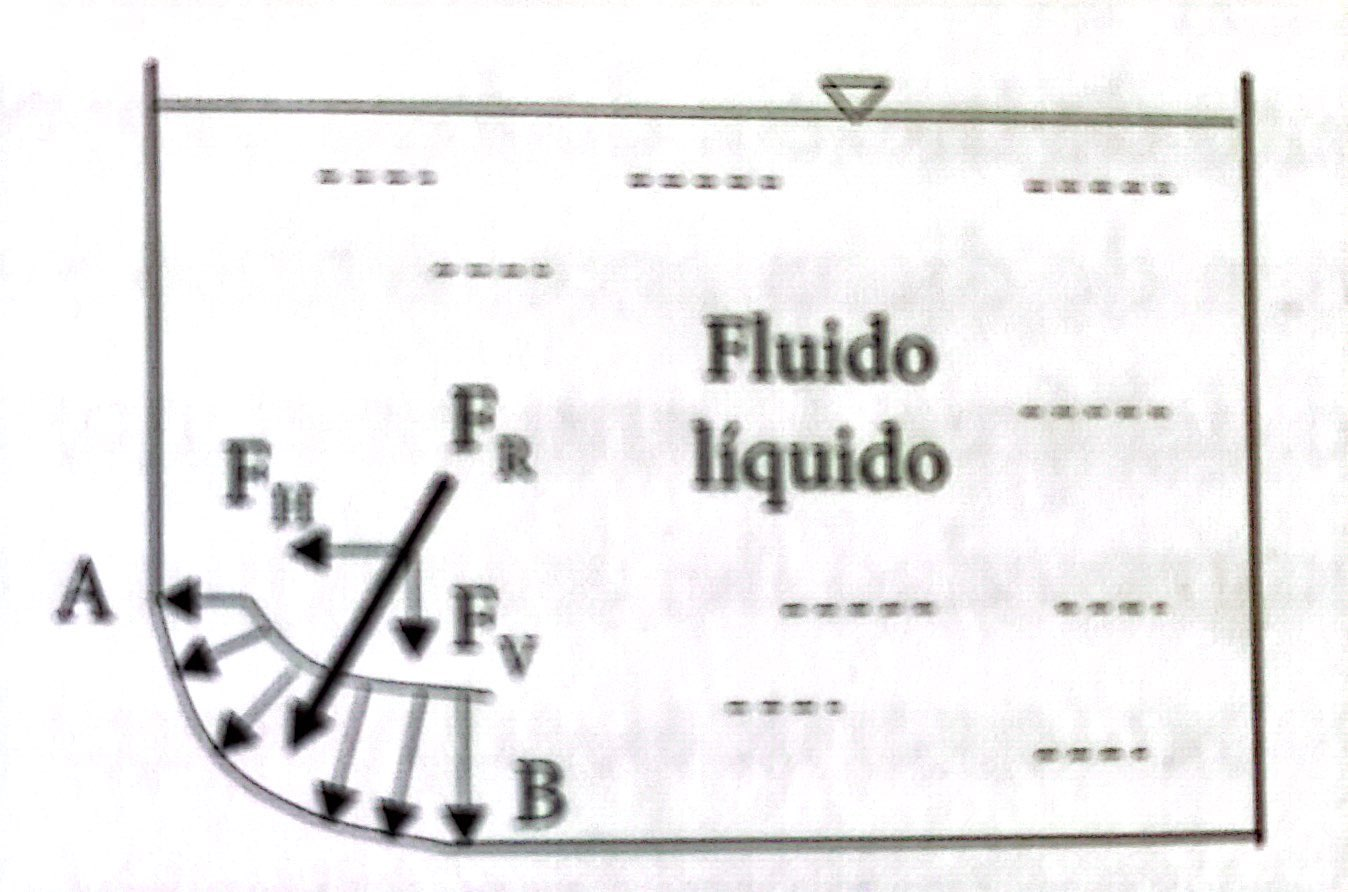
\includegraphics[width=\textwidth]{curb2}
\end{textblock*}
\end{frame}

\begin{frame}{Fuerzas sobre superficies curvas: $F_H$}
\begin{columns}
\column{0.4\textwidth}
La fuerza horizontal $F_H$ sobre la proyecci\'on de la superficie curva es:
$$
F_H=\gamma[h_c A]_{\text{proyecci\'on}} 
$$
\column{0.6\textwidth}
\begin{textblock*}{6cm}(6.8cm,1cm) % {block width} (coords)
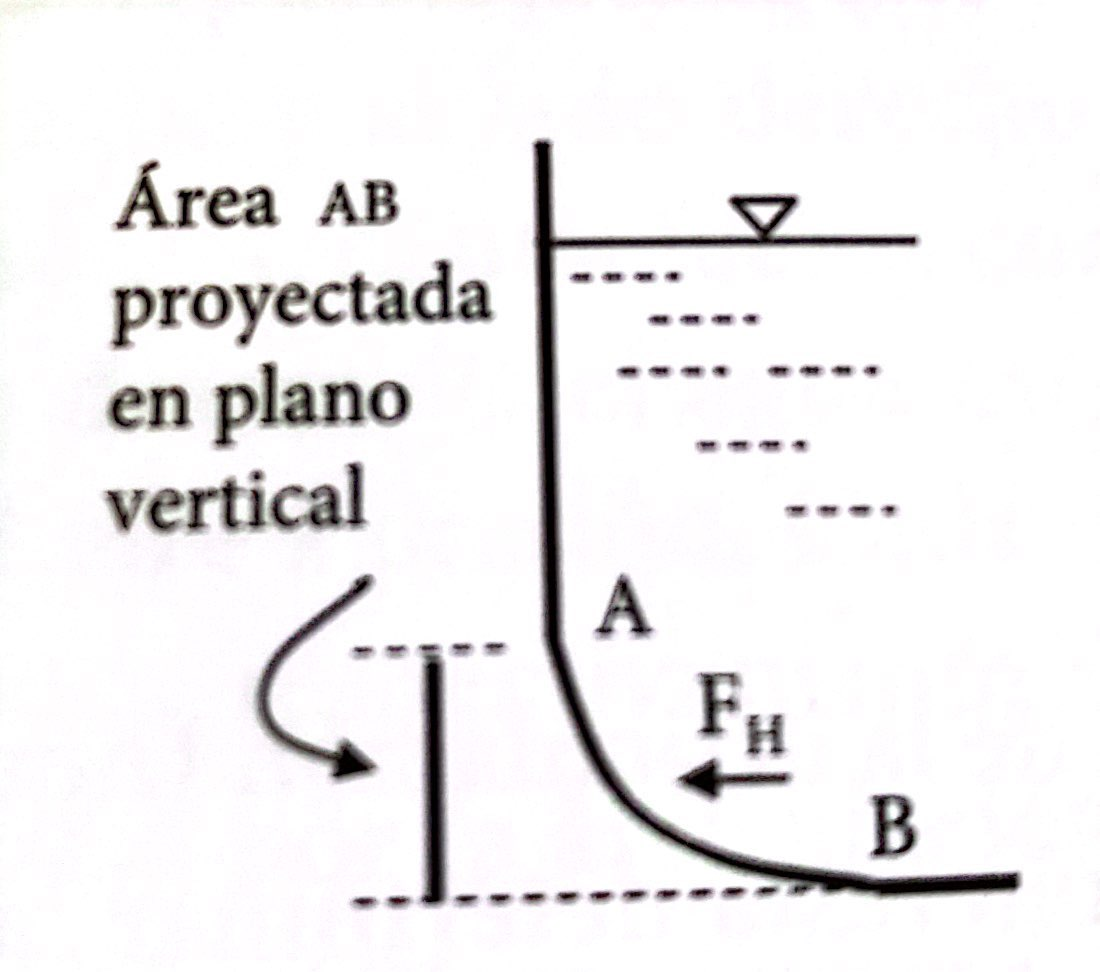
\includegraphics[width=0.9\textwidth]{curb3}
\end{textblock*}
\end{columns}
\vspace{1.5cm}
donde:
\begin{itemize} 
\item $\gamma$: Peso espec\'ifico del fluido en reposo.
\item $h_c$: distancia vertical medida desde la superficie hasta el centro de gravedad de la superficie proyectada
\item $A$: \'Area de la superficie proyectada sobre el plano vertical.
\end{itemize}
\end{frame}

\begin{frame}{Fuerzas sobre superficies curvas:$y_p$ y $x_p$ para $F_H$}
Como $F_H$ se aplica en el centro de presiones $p$ del \'area proyectada en un plano vertical, se tiene:
$$
y_p = \left[ y_c + \frac{\bar{I}_c}{y_c A} \right]_{\text{proyecci\'on}}
$$

$$
x_p = \left[ x_c + \frac{\bar{I}_{xy}}{x_c A} \right]_{\text{proyecci\'on}}
$$
donde
\begin{itemize}
\item $\bar{I}_c$: Momento de inercia con respecto al centro de gravedad del \'area proyectada en un plano vertical.
\item $\bar{I}_{xy}$: Producto de inercia con respecto al centro de gravedad del \'area proyectada en un plano vertical.
\item $x_c$ y $y_c$ son las coordenadas del centro de gravedad del \'area proyectada en un plano vertical.
\end{itemize}
\end{frame}

\begin{frame}{Fuerzas sobre superficies curvas: $F_V$}
\begin{columns}
\column{0.6\textwidth}
La componente vertical $F_V$ se calcula como el peso del fluido que esta por encima (f\'isicamente o no). 
$$
F_V = \gamma [V]_{arriba}
$$
\column{0.4\textwidth}
\begin{textblock*}{3cm}(8cm,1.1cm) % {block width} (coords)
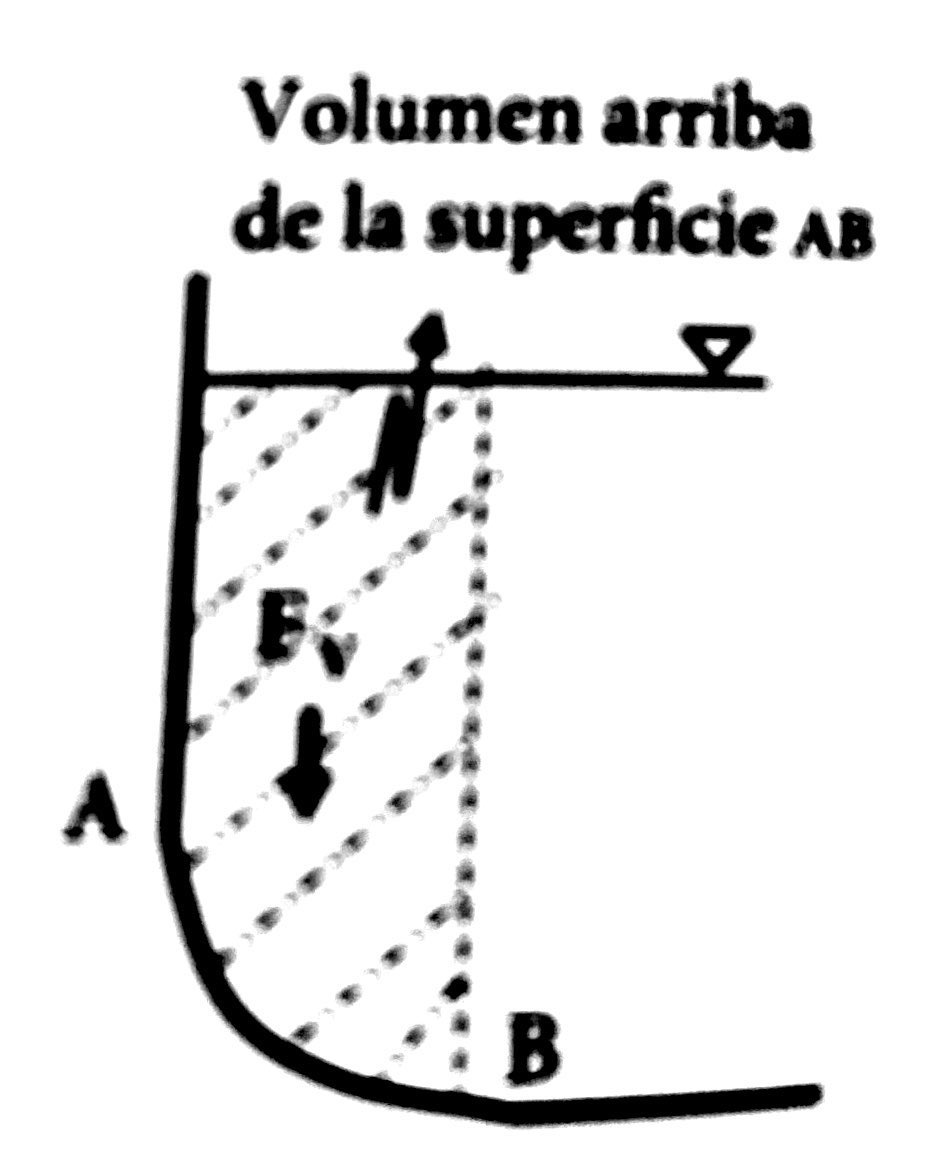
\includegraphics[width=0.9\textwidth]{curb4}
\end{textblock*}
\end{columns}
\vspace{0.8cm}
El punto de aplicaci\'on de $F_V$ es el centro de gravedad del volumen situado arriba de la superficie curva:
$$
y_p = [y_c ]_{V_{arriba}} = \frac{\int_V y dV}{\int_V dV}
$$
$$
x_p = [x_c ]_{V_{arriba}}= \frac{\int_V x dV}{\int_V dV}
$$
Finalmente,la magnitud de la fuerza $F_R$ se calcula como:
$$
\sqrt{F_H^2 + F_V^2}
$$
\end{frame}

%\item $F_x$ se calcula como la resultante de la fuerza hidroestatica sobre una superficie plana vertical $F_x = \gamma\ h_c \ A$
%\item $F_y$ es la fuerza en $y$ ejercida sobre el fluido (e.g. fluido superior y aire) 
%\item $W = \rho g V$ es el peso del volumen ($V$) de fluido. Note que $F_y$ y $W$ se suman si actuan en la misma direccion y se restan si van en direcciones opuestas. 
%\end{itemize}
%$F_R$ se calcula como:
%$$
%F_R=\sqrt{F^2_H + F^2_V}
%$$
%El angulo que hace $F_R$ con la horizontal es:
%$$$
%\alpha = \arctan \frac{F_V}{F_H}
%$$

\section{Fuerzas hidroest\'aticas con diferentes fluidos}
\begin{frame}{Fuerzas hidroest\'aticas con diferentes fluidos}
\begin{columns}
\column{0.4\textwidth}
Las ecuaciones  vistas hasta le momento son v\'alidas para fluidos de densidad uniforme. Si el fluido esta conformado por capas de fluidos de diferentes densidades, la distribuci\'on lineal de presiones cambia en cada capa. 
% Fig 3.39 Cengel
\column{0.6\textwidth}
\begin{textblock*}{6cm}(6cm,1.5cm) % {block width} (coords)
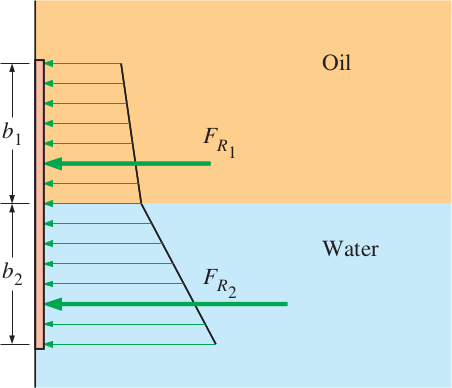
\includegraphics[width=\textwidth]{mden}
\end{textblock*}
\end{columns}
\end{frame}

\begin{frame}{Fuerzas hidroest\'aticas con diferentes fluidos}
Sin embargo las ecuaciones vistas anteriormente pueden ser aplicadas a cada capa $i$ y las $F_{R,i}$ pueden ser adicionadas para calcular la $F_R$:
$$
F_R = \sum F_{R,i} = \sum P_{C,i}A_i
$$
dondei: 
\begin{itemize}
\item $P_{C,i} =  P_0 + \rho_i h_{C,i}$ es la presi\'on en el centroide de la porci\'on de la superficie en el fluido $i$.
\item $A_i$ es el \'area de la superficie en ese fluido. El centro de presi\'on de $F_R$ puede ser encontrado calculando la suma de los momentos de cada fuerza $F_{R,i}$ con respecto a un punto determinado (e.g. la superficie de agua).
\end{itemize}
$$
y_p = \frac{\sum F_{R,i}\ y_{p,i}}{F_R} \hspace{1cm} x_p = \frac{\sum F_{R,i}\ x_{p,i}}{F_R}
$$
\end{frame}

\section{Flotaci\'on y estabilidad}
\begin{frame}{Flotaci\'on y estabilidad: Introducci\'on}
\begin{columns}
\column{0.5\textwidth}
\begin{block}{Fuerza de flotaci\'on}
La \emph{fuerza de flotaci\'on ($F_B$)} es una fuerza vertical hacia arriba que ejerce un fluido sobre un cuerpo sumergido, la cual tiende a levantar el cuerpo. Esta fuerza es causada por el incremento de la presi\'on con la profundidad. Por esto, es com\'un sentir que un cuerpo pesa menos cuando este est\'a en un fluido.
\end{block}
\column{0.5\textwidth}
\begin{textblock*}{6cm}(6.5cm,2cm) % {block width} (coords)
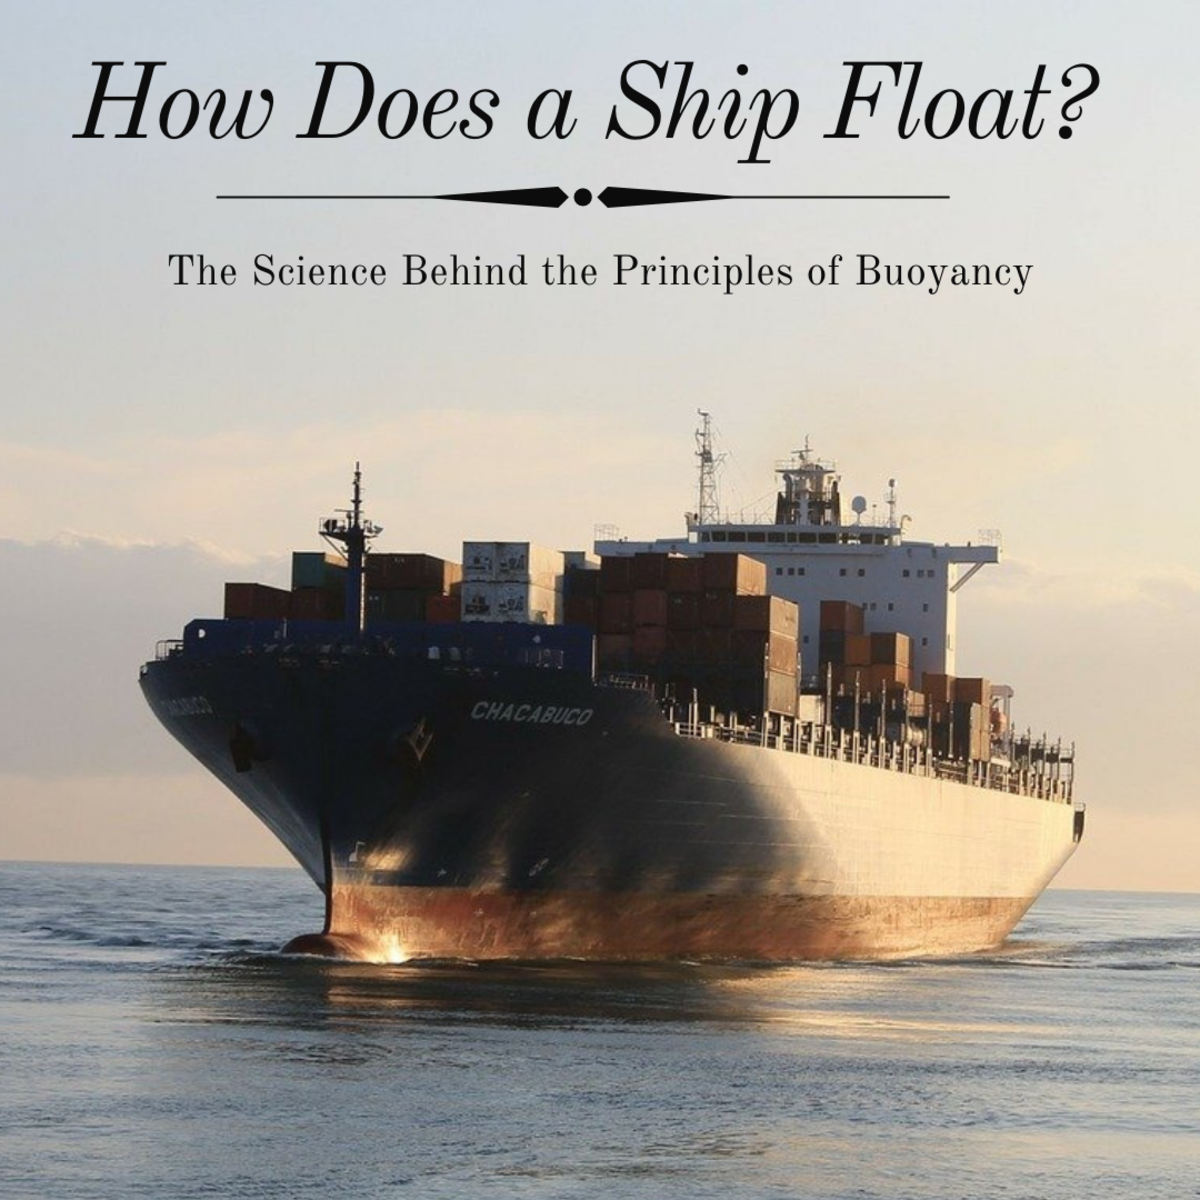
\includegraphics[width=\textwidth]{buoy}
\end{textblock*}
\end{columns}
\end{frame}
%Es comun sentir como un cuerpo determinado pesa menos cuando este esta en un fluido; dicha sensacion se explica debido a que el fluido ejerce una fuerza vertical hacia arriba que tiende a levantar el objeto la cual es denominada \textbf{fuerza de flotaci\'on}, $F_B$. La fuerza de flotaci\'on es causada por el incremento de presion con la profundidad dentro del fluido. Para su analisis, consideremos la placa de la figura~\ref{flota} de espesor $h$ y area $A$ sumergida en un liquido de densidad $\rho_f$ y que es paralela a la superficie libre. El balance de fuerzas sobre la placa, con base en presiones manometricas es:
% Fig 3.41 Cengel

\begin{frame}{Flotaci\'on y estabilidad: Fuerza de flotaci\'on}
\begin{columns}
\column{0.5\textwidth}
Consideremos una placa de espesor $h$ y are\'a $A$ sumergida en un liquido de densidad $\rho$ y que es paralela a la superficie libre. El balance de fuerzas sobre la placa, con base en presiones manom\'etricas es:

\column{0.5\textwidth}
\begin{textblock*}{5cm}(7.5cm,1cm) % {block width} (coords)
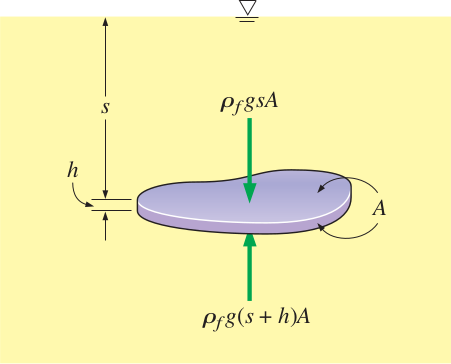
\includegraphics[width=\textwidth]{flota}
\end{textblock*}
\end{columns}
\vspace{1.1cm}
$$
F_B=F_{bottom} - F_{top} = \rho g (s+h)A - \rho gs A = \rho ghA = \rho g V
$$
donde $V=hA$ es el volumen de la placa.\\ 
\begin{block}{}
Teniendo en cuenta que $\rho g V$ es el peso del liquido cuyo volumen es igual al volumen de la placa, tenemos que \emph{la fuerza de flotaci\'on actuante sobre una placa es igual al peso del liquido desplazado por la placa}. Note que si el fluido es de densidad constante, la fuerza de flotacion es independiente de la profundidad $h$ y  de la densidad de la placa. 
\end{block}

\end{frame}

\begin{frame}{Flotaci\'on y estabilidad: Principio de Arqu\'imides}
\vspace{-0.5cm}
\begin{block}{Principio de Arqu\'imidez}
\emph{La fuerza de flotaci\'on actuante sobre un cuerpo de densidad uniforme inmerso en un fluido es igual al peso del fluido desplazado por el cuerpo, y que actual vertical a trav\'ez del centroide del volumen desplazado}, esto es conocido como el \textbf{principio de Arqu\'imides} gracias al matem\'atico Griego Arqu\'imides. 
Para objetos flotantes, el peso del cuerpo debe ser igual a la fuerza de flotaci\'on, la cual es el peso del fluido cuyo volumen es igual a el volumen de la porci\'on sumergida del cuerpo flotante. Esto es:
$$
F_B = W \rightarrow \rho g V_{sub} = \rho_{body}gV_{total} \rightarrow \frac{V_{sub}}{V_{total}} = \frac{\rho_{body}}{\rho}
$$
Tenemos entonces que la fracci\'on de volumen del objeto flotante es igual a la relaci\'on entre la densidad promedio del cuerpo y la densidad del fluido. 
\end{block}
\end{frame}

\begin{frame}{Flotaci\'on y estabilidad: Principio de Arqu\'imides}
\begin{columns}
\column{0.5\textwidth}
Analizando la ecuaci\'on anterior, un objeto inmerso en un fluido: 
\begin{enumerate}
\item permanece en reposo dentro del fluido cuando $\rho = \rho_f$
\item se hunde y cae hasta el fondo dentro de el fluido cuando $\rho > \rho_f$ 
\item flota cuando $\rho < \rho_f$
\end{enumerate}
\column{0.5\textwidth}
\begin{textblock*}{6cm}(6.5cm,1cm) % {block width} (coords)
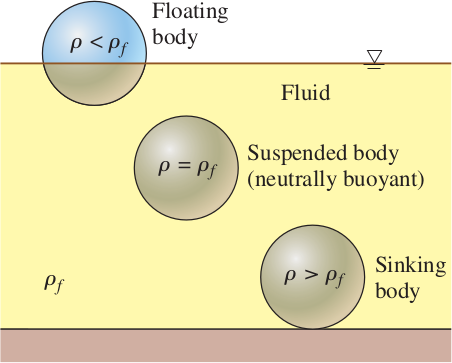
\includegraphics[width=\textwidth]{flota2}
\end{textblock*}
\end{columns}
\vspace{0.5cm}
En el caso de los gases, la densidad generalmente es mucho menor que la densidad de un liquido. Sin embargo, las fuerzas de flotaci\'on son notorias en el ascenso de aire caliente en ambientes frios, la circulaci\'on de aire en la atm\'osfera y el ascenso de globos y de bombas con helio. 
\end{frame}

\subsection{Estabilidad de cuerpos sumergidos y flotantes}
\begin{frame}{Estabilidad de cuerpos sumergidos y flotantes}
Una importante aplicaci\'on del concepto de flotaci\'on es el an\'alisis de la estabilidad de un cuerpo flotante o sumergido, lo cual es fundamental en el disen\~o de embarcaciones y submarinos. Existen tres casos que describen la estabilidad de un cuerpo: 
\begin{itemize}
\item un cuerpo permanece \textbf{estable} si cualquier peque\~na perturbaci\'on genera un movimiento que es contrarestado por una fuerza que hace que el cuerpo retorne a su posici\'on inicial
\item un cuerpo es \textbf{neutralmente estable} si despu\'es de ser perturbado cambia su posici\'on inicial
\item un cuerpo es \textbf{inestable} si al ser perturbado este no retorna a su posici\'on inicial y continua en movimiento. 
\end{itemize}
Estos tres estados son aplicables a objetos flotantes o sumergidos. Por ejemplo, un cuerpo sumergido o flotante en equilibrio est\'atico cuyo peso es balanceado por la fuerza de flotaci\'on permanece estable en la \textbf{direcci\'on vertical}.
\end{frame}

\begin{frame}{Estabilidad de cuerpos sumergidos y flotantes}
\small
\vspace{-0.8cm}
\begin{columns}
\column{0.6\textwidth}
\begin{block}{Estabilidad de rotaci\'on}
La \textbf{estabilidad de rotaci\'on} de un cuerpo cuerpo sumergido depende de la localizaci\'on relativa de el \textbf{centro de gravedad} $G$ de el cuerpo y el centro de flotaci\'on $B$, el cual es el centroide del volumen desplazado. 
\begin{enumerate}
\item Un cuerpo sumergido permanece estable si su fondo es m\'as pesado lo que hace que $G$ este por debajo de $B$ (e.g. motores en submarinos, canasta en globos) 
\item En el caso en el que $G$ y $B$ coinciden, el cuerpo sumergido es neutralmente estable, lo cual es el caso de cuerpos cuya densidad es uniforme.
\item Si $G$ esta por encima de $B$, el cuerpo sumergido es inestable y cualquier perturbaci\'on hace que el cuerpo se voltee. 
\end{enumerate}
\end{block}
\column{0.3\textwidth}
\begin{textblock*}{4cm}(8.5cm,1cm) % {block width} (coords)
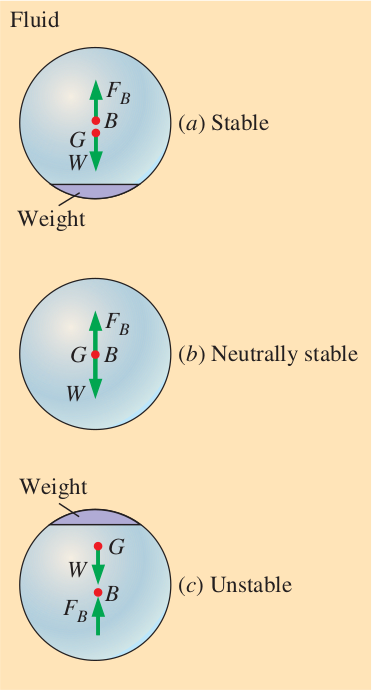
\includegraphics[width=\textwidth]{rota}
\end{textblock*}
\end{columns}
\end{frame}

\begin{frame}{Estabilidad de cuerpos sumergidos y flotantes}
\begin{block}{Momento restaurador}
\begin{columns}
\column{0.6\textwidth}
Si en un cuerpo $G$ no esta verticalmente alineado con $B$ no es apropiado hablar de estabilidad ya que el cuerpo no esta en un estado de equilibrio y tratara de rotar o moverse por si solo para alcanzar su estado estable. El \emph{momento restaurador} que act\'ua en contra de las manecillas del reloj, tratar\'a de rotar el cuerpo en la misma direcci\'on con el fin de alinear $G$ y $B$ verticalmente.
\column{0.4\textwidth}
\begin{textblock*}{5cm}(7.5cm,2.3cm) % {block width} (coords)
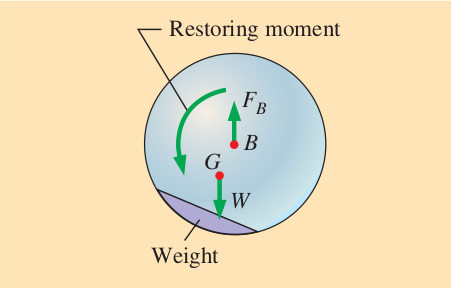
\includegraphics[width=\textwidth]{rota2}
\end{textblock*}
\end{columns}
\end{block}
\end{frame}

\begin{frame}{Estabilidad de cuerpos sumergidos y flotantes}
\begin{block}{Estabilidad de rotaci\'on}
La estabilidad de rotaci\'on es similar para cuerpos flotantes. Sin embargo, a diferencia de un cuerpo sumergido, un cuerpo flotante puede permanecer estable incluso cuando $G$ esta arriba de $B$. Esto se logra gracias a que $B$ se desplaza hacia $B'$ generando un momento restaurador entre las dos fuerzas para retornar el objeto a su posici\'on  original. 
\begin{textblock*}{8cm}(2.5cm,5cm) % {block width} (coords)
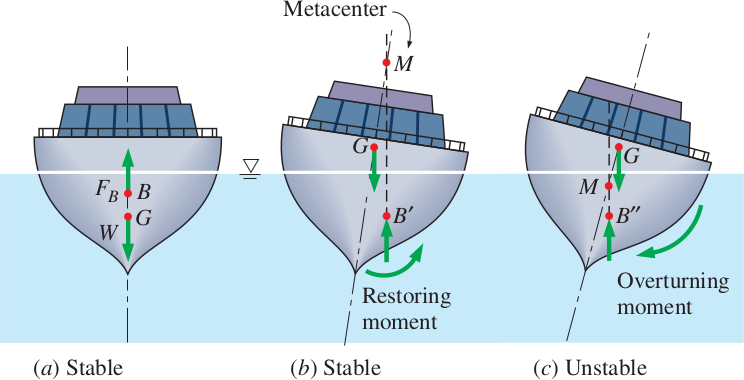
\includegraphics[width=\textwidth]{rota3}
\end{textblock*}
\end{block}
\end{frame}

\begin{frame}{Estabilidad de cuerpos sumergidos y flotantes}
\small
\vspace{-0.5cm}
\begin{block}{Altura metacentrica}
Una medida de la estabilidad de un cuerpo flotante es la \textbf{altura metacentrica} $GM$, la cual es la distancia entre $G$ y el \emph{metacentro} $M$ (punto de intersecci\'on entre la linea de acci\'on de las fuerza flotante antes y despu\'es de la rotaci\'on). Con base en la posici\'on de $M$, un cuerpo flotante es estable si $M$ esta arriba de $G$ por lo que $GM$ es positiva y es inestable si $M$ esta abajo de $G$ por lo que $GM$ es negativa. Si es inestable, el peso y la fuerza de flotaci\'on actuando sobre el cuerpo inclinado genera un momento de volcamiento en lugar de un momento restaurador. Entre m\'as grande es $GM$, m\'as estable es el cuerpo flotante. Note que un bote puede inclinarse hasta cierto angulo m\'aximo sin volcarse, sin embargo, si dicho \'angulo es excedido el bote se voltear\'a y se hundir\'a.  
\begin{textblock*}{5cm}(4.2cm,6cm) % {block width} (coords)
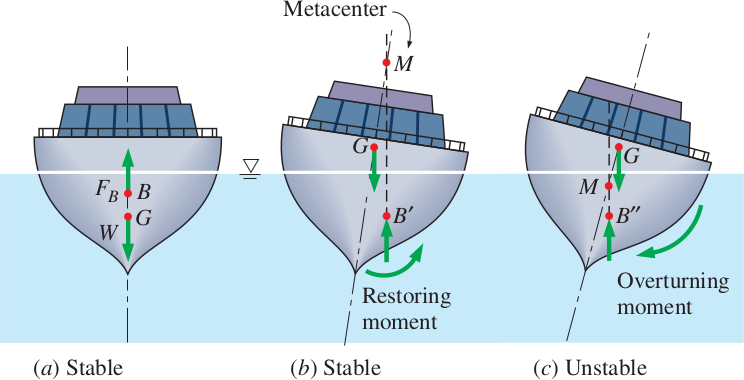
\includegraphics[width=\textwidth]{rota3}
\end{textblock*}
\end{block}
\end{frame}



\section{Equilibrio relativo de fluidos en movimiento}
\begin{frame}{Equilibrio relativo de fluidos en movimiento}
Se analizan las variaciones de presi\'on en un fluido que se mueve como un cuerpo s\'olido con o sin aceleraci\'on o sin la presencia de esfuerzos cortantes. Ejemplos:
\begin{itemize}
\item Un carrotanque que transporta l\'iquido en su interior, al acelerar y alcanzar una velocidad, hace que la superficie libre de el fluido se incline en la parte trasera haciendo que el volumen se mueva como un cuerpo r\'igido. 
\item De manera similar, cuando un cilindro que contiene un fluido rota a una velocidad determinada, su superficie se transforma haciendo que todo el fluido se comporte como un cuerpo r\'igido.
\end{itemize}
% Figura de carrotante
% FIgura de tanque en rotaci\'on
\end{frame}

\begin{frame}{Equilibrio relativo de fluidos en movimiento}
\footnotesize
\vspace{-0.4cm}
\begin{columns}
\column{0.6\textwidth}
Si analizamos un elemento diferencial de fluido cuyas dimensiones son $dx$, $dy$ y $dz$  el cual se comporta como un cuerpo r\'igido, la fuerza neta actuante sobre el elemento seg\'un la \emph{segunda ley de Newton} se expresa como:
$$
\delta \vec{F} = \delta m \cdot \vec{a}
$$
donde $\delta m = \rho\ dV = \rho\ dx\ dy\ dz$ es la masa del elemento de fluido y $\vec{a}$ es la aceleraci\'on del elemento. 
Si hacemos un balance de fuerzas sobre el elemento, las fuerzas actuantes sobre este son las fuerzas hidroest\'aticas sobre las caras del elemento  y el peso del elemento en direcci\'on $z$ negativo.
\column{0.4\textwidth}
% Fig 3.53 Cengel
\begin{textblock*}{5cm}(7.6cm,1cm) % {block width} (coords)
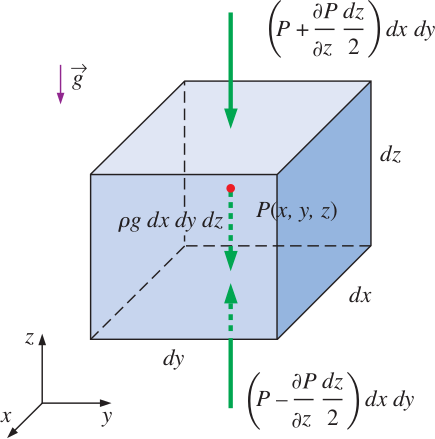
\includegraphics[width=\textwidth]{body}
\end{textblock*}
\end{columns}
\vspace{0.5cm}
El balance de las fuerzas de presi\'on en la direcci\'on $z$ es:
$$
\delta F_{S,z} = \left( P - \frac{\partial P}{\partial z} \frac{dz}{2} \right) dx\ dy - \left( P + \frac{\partial P}{\partial z} \frac{dz}{2} \right) dx\ dy = -\frac{\partial P}{\partial z} dx\ dy\ dz
$$
De manera similar, el balance en la direcci\'on $x$ y $y$ es:
$$
\delta F_{S,x} =  -\frac{\partial P}{\partial x} dx\ dy\ dz \quad \quad  \delta F_{S,x} =  -\frac{\partial P}{\partial x} dx\ dy\ dz
$$
\end{frame}

\begin{frame}{Equilibrio relativo de fluidos en movimiento}
La fuerza de presi\'on actuando sobre el elemento en forma vectorial, es expresada como:
\begin{align*}
\delta \vec{F}_S = \delta F_{S,x}\vec{i} + \delta F_{S,y} \vec{j} + \delta F_{S,z}\vec{k} &= -\left( \frac{\partial P}{\partial x}\vec{i} + \frac{\partial P}{\partial y}\vec{j} + \frac{\partial P}{\partial z}\vec{k} \right) dx\ dy\ dz \\
&= -\vec{\nabla}P dx\ dy\ dz
\end{align*}
donde $\vec{i}$, $\vec{j}$ y $\vec{k}$ son los vectores unitarios en $x$, $y$ y $z$ respectivamente, y $\vec{\nabla}= \frac{\partial P}{\partial x}\vec{i} + \frac{\partial P}{\partial y}\vec{j} + \frac{\partial P}{\partial z}\vec{k}$ es el gradiente de presi\'on. Note que $\vec{\nabla}$ es un operador vectorial que act\'ua sobre una funci\'on escalar como lo es $P$.

La otra fuerza actuante sobre el elemento de fluido es el peso, la cual se expresa como:
$$
\delta \vec{F}_{B,z} = -g \delta m \vec{k} = -\rho g dx\ dy\ dz \vec{k}
$$
La fuerza total actuante sobre el elemento de fluido es:
$$
\delta \vec{F} = \delta \vec{F}_S + \delta \vec{F}_B = -\left( \vec{\nabla}P + \rho g \vec{k}\right) dx\ dy\ dz
$$
\end{frame}

\begin{frame}{Equilibrio relativo de fluidos en movimiento}
De acuerdo con la segunda ley de Newton, $\delta \vec{F} = \delta m \cdot \vec{a} = \rho\ dx\ dy\ dz$ y substituyendo en la ecuaci\'on anterior, tenemos que la ecuaci\'on general de movimiento de un fluido que act\'ua como un cuerpo r\'igido (sin esfuerzos cortantes) es:
$$
\vec{\nabla}P + \rho g \vec{k} = -\rho \vec{a}
$$
Descomponiendo la ecuaci\'on vectorial, tenemos:
$$
\frac{\partial P}{\partial x} = -\rho a_x \quad \frac{\partial P}{\partial y} = -\rho a_y \quad \frac{\partial P}{\partial z} = -\rho (g+ a_z )
$$
donde $a_x$, $a_y$ y $a_z$ son las componentes del vector $\vec{a}$ en las direcciones $x$, $y$ y $z$ respectivamente.
\end{frame}

\begin{frame}{Equilibrio relativo de fluidos en movimiento}
\small
\vspace{-0.4cm}
Existen dos casos especiales:
\begin{enumerate}
\item \textbf{Fluido en reposo o en movimiento a velocidad constante:}
En un fluido en reposo o en movimiento con velocidad constante, $a_x=0$, $a_y=0$ y $a_z=0$, la equaci\'on general se reduce a:
$$
\frac{d P}{d z} = -\rho g
$$
La ecuaci\'on anterior confirma que en un fluido en reposo, la presi\'on permanece constante en cualquier direcci\'on horizontal y solo varia en la direcci\'on vertical.

\item \textbf{Ca\'ida libre de un elemento fluido}: Para un cuerpo en ca\'ida libre cuya aceleraci\'on es $a_x =0$, $a_y =0$ y $a_z = -g$ y en donde la resistencia del aire despreciable, la ecuaci\'on general se convierte en:
$$
\frac{\partial P}{\partial x} =\frac{\partial P}{\partial y} =\frac{\partial P}{\partial z} = 0 \rightarrow P=\text{constant} \rightarrow a_z=-g
$$
Si el cuerpo es acelerado hacia arriba (e.g. un elemento de fluido en un ascensor) hasta alcanzar $a_z = g$, el gradiente de presi\'on en direcci\'on $z$, de acuerdo con la ecuaci\'on general, es $\partial P \ \partial z = -2\rho ga$.
\end{enumerate}
\end{frame}

\subsection{Aceleraci\'on en l\'inea recta}
\begin{frame}{Aceleraci\'on en l\'inea recta}
\begin{columns}
\column{0.5\textwidth}
Consideremos un contenedor parcialmente lleno moviendose en linea recta con una aceleraci\'on constante (e.g. carrotanque con combustible en movimiento). De acuerdo con la figura y con la ecuaci\'on general, las ecuaciones de  movimiento se reducen a:
\column{0.5\textwidth}
% Fig 3.57 Cengel
\begin{textblock*}{4cm}(7.6cm,1cm) % {block width} (coords)
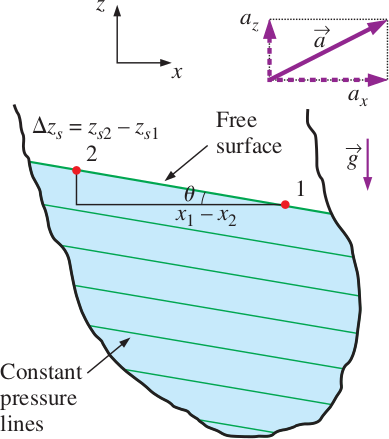
\includegraphics[width=\textwidth]{rigi}
\end{textblock*}
\end{columns}
\vspace{0.5cm}
$$
\frac{\partial P}{\partial x}=-\rho a_x \quad \frac{\partial P}{\partial y} = 0 \quad \frac{\partial P}{\partial z}=-\rho(g+ a_z)
$$
en donde $P$ es independiente de $y$ por lo cual $P=P(x,z)$. De acuerdo con la definici\'on de diferencial total, $dP = (\partial P / \partial x)dx + (\partial P / \partial z)dz$, la ecuaci\'on anterior se convierte en:
$$
dP = -\rho a_x dx - \rho(g + a_z)dz
$$
\end{frame}

\begin{frame}{Aceleraci\'on en l\'inea recta}
\vspace{-0.4cm}
Para determinar la diferencia de presi\'on entre los puntos 1 y 2 (ver figura), integramos la ecuaci\'on para $x$ y $z$:
\begin{center}
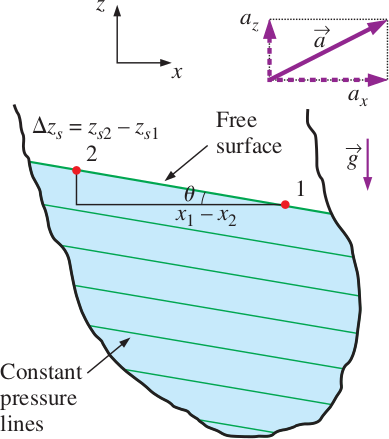
\includegraphics[width=0.3\textwidth]{rigi}
\end{center}
$$
P_2 - P_1 = -\rho a_x (x_2 - x_1 ) - \rho(g+ a_z )(z_2 - z_1 )
$$
%\begin{textblock*}{4cm}(7.6cm,1cm) % {block width} (coords)
%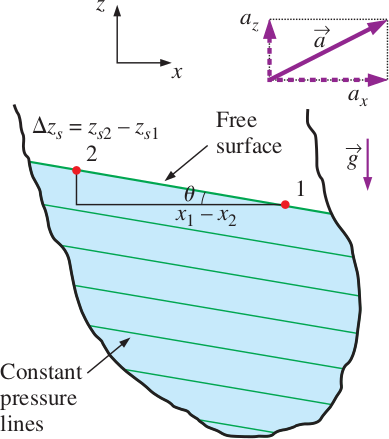
\includegraphics[width=\textwidth]{rigi}
%\end{textblock*}
Si tomamos como origen el punto $x=0$ y $z=0$ en donde la presi\'on $P=P_0$, la variaci\'on de presi\'on en cualquier punto del fluido es:
$$
P = P_0 - \rho a_x x - \rho(g + a_z) z
$$
\end{frame}

\begin{frame}{Aceleraci\'on en l\'inea recta}
\vspace{-0.4cm}
Si deseamos calcular el c\'ambio de elevaci\'on de la superficie libre del fluido, el c\'ambio de nivel del punto 2 con respecto a 1 de acuerdo a la ecuaci\'on y asumiendo que $P_1 = P_2$ es:
\vspace{0.5cm}
\begin{textblock*}{2.8cm}(9.6cm,2.5cm) % {block width} (coords)
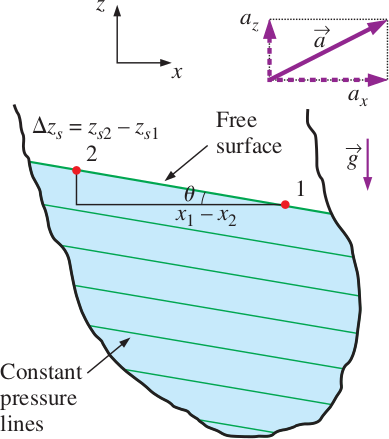
\includegraphics[width=\textwidth]{rigi}
\end{textblock*}
\begin{flalign*}
&\Delta z_s = z_{s2} - z_{s1} = -\frac{a_x}{g+a_z} (x_2 - x_1)&
\end{flalign*}
\vspace{0.8cm}
donde $z_s$ indica la localizaci\'on sobre la superficie. 

De manera similar, las superficies con presi\'on constante conocidas como \textbf{isobaras} pueden ser descritas como:
$$
\frac{d z_{isobar}}{dx} = -\frac{a_x}{g+a_z} = \text{constante}
$$
De acuerdo con lo anterior, las isobaras son superficies paralelas (ver figura) cuya pendiente es $m = \frac{dz_{isobar}}{dx} = -\frac{a_x}{g+ a_z } = \tan \theta$.
\end{frame}
\subsection{Rotaci\'on de un contenedor cil\'indrico}
\begin{frame}{Rotaci\'on de un contenedor cil\'indrico}
\vspace{-0.4cm}
\small
\begin{columns}
\column{0.6\textwidth}
Si hacemos rotar un vaso lleno de agua alrededor de su eje vertical, el agua tiende a apartarse desde el centro hacia las paredes formando una superficie libre c\'oncava; todo esto gracias a la \emph{fuerza centrifuga} (o a la \emph{aceleraci\'on centripeta}). Si analiz\'amos el cilindro de la figura, el cual rota a velocidad angular $\omega$,  cada particula del fluido se mover\'a a la misma velocidad y todo el fluido se mover\'a como un cuerpo r\'igido que no se deforma, una vez se alcance una condici\'on permanente. Para analizar este caso, es conveniente el an\'alisis en coordenadas pol\'ares ($r$, $\theta$, $z$), en donde $z$ represente el eje de rotaci\'on del fluido. Por definici\'on, la aceleraci\'on centripeta es $r \omega^2$ y positiva hacia el centro; note que la aceleraci\'on no depende de $\theta$ ya que es sim\'etrica con respecto a $z$. 
\column{0.4\textwidth}
\vspace{-0.4cm}
% Fig 3.59 Cengel
\begin{center}
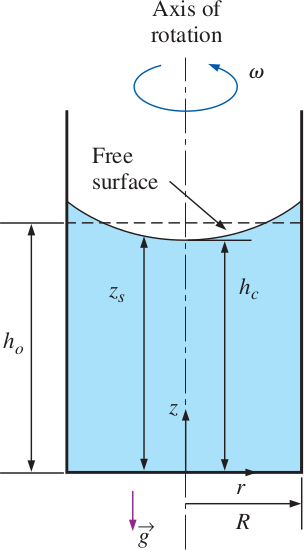
\includegraphics[width=4cm]{cili}
\end{center}
\end{columns}
\end{frame}

\begin{frame}{Rotaci\'on de un contenedor cil\'indrico}
\vspace{-0.4cm}
\footnotesize
Aplicando la ecuaci\'on general:
$$
\frac{\partial P}{\partial r} = \rho r \omega^2 \quad \frac{\partial P}{\partial \theta} = 0 \quad \frac{\partial P}{\partial z} = -\rho g
$$
De acuerdo con la definici\'on de diferencial total, $dP = (\partial P / \partial r)dr + (\partial P / \partial z)dz$, la ecuaci\'on anterior se convierte en:
$$
dP = \rho r \omega^2 dr - \rho g dz
$$
Para superficies con presi\'on constante ($dP = 0$), la distancia vertical $z$ se convierte en una funci\'on de $r$ como:
$$
\frac{d z_{isobar}}{dr} = \frac{r \omega^2}{g}
$$
integrando la ecuaci\'on anterior:
\vspace{-0.4cm}
$$
z_{isobar} = \frac{\omega^2}{2g} r^2 + C_1
$$
en donde la ecuaci\'on anterior es la ecuaci\'on de la par\'abola por lo que las superficies de presi\'on constante forman un parabol\'oide de revoluci\'on. La ecuaci\'on anterior representa una familia de curvas. Por lo tanto, para la superficie libre, cuya altura es conocida e igual a $h_c$, $C_1=h_c$ cuando $r=0$ y la ecuaci\'on anterior para la superficie libre se convierte en:
\vspace{-0.3cm}
$$
z_s = \frac{\omega^2}{2g} r^2 + h_c
$$
en donde $z_s$ es la distancia desde el fondo hasta la superficie. 
\end{frame}

\begin{frame}{Rotaci\'on de un contenedor cil\'indrico}
\vspace{-0.4cm}
\footnotesize
Teniendo en cuenta que el volumen de un anillo es $dV = 2\pi r z_s dr$, el volumen del parabol\'odide formado por la superficie libre es:
$$
V = \int_{r=0}^R 2\pi z_s r dr = 2\pi \int_{r=0}^R \left( \frac{\omega^2}{2g} r^2 + h_c \right) r dr = \pi R^2 \left( \frac{\omega^2}{2g} R^2 + h_c \right)
$$
De acuerdo con el principio de conservaci\'on de la masa, el volumen del cilindro es:
$$
V=\pi R^2 h_0
$$
en donde $h_0$ es la altura del fluido en el contenedor antes de rotar. Igualando las ecuaciones anteriores, $h_c$ se convierte en:
$$
h_c = h_0 - \frac{\omega^2 R^2}{4g}
$$
reemplazando en la ecuaci\'on, la altura de la superficie libre ser\'ia:
$$
z_s = h_0 - \frac{\omega^2}{4g} ( R^2 -2r^2 )
$$
La diferencia de altura entre el centro y el borde del contenedor se obtiene evaluando la ecuaci\'on anterior cuando $r=0$ y $r=R$:
$$
\Delta z_{s,max} = z_s (R)- z_s (0) = \frac{\omega^2}{2g} R^2
$$
\end{frame}

\begin{frame}{Rotaci\'on de un contenedor cil\'indrico}
\vspace{-0.4cm}
\footnotesize
Por otro lado, si la densidad $\rho$ es constante, la diferencia de presi\'on entre dos puntos 1 y 2 se determina integrando la ecuaci\'on general, lo cual queda:
$$
P_2 - P_1 = \frac{\rho \omega^2}{2}(r_2^2 - r_1^2 ) - \rho g (z_2 - z_1)
$$
Si tomamos como punto 1 $r=0$ y $z=0$ donde la presi\'on es igual $P_0$, la presi\'on en cualquier punto (e.g. $P_2$) es:
$$
P = P_0 + \frac{\rho \omega^2}{2} r^2 - \rho g z 
$$

Seg\'un la ecuaci\'on anterior, para un radio conocido, $P$ varia hidroest\'aticamente en la direcci\'on vertical como un fluido en reposo. Por otro lado, para una distancia $z$ conocida, $P$ cambia con el cuadrado de $r$ e incrementa desde el centro hacia los bordes. La diferencia de presi\'on entre el centro y el borde del contenedor es:
$$
\Delta P = \frac{\rho \omega^2}{2} R^2 
$$
\end{frame}
\end{document}

